\documentclass[tikz,border=15pt]{standalone}
\usepackage[utf8]{inputenc}
\usepackage[T5]{fontenc}
\usetikzlibrary{shapes.multipart, arrows.meta, positioning, calc, backgrounds, fit}

\begin{document}
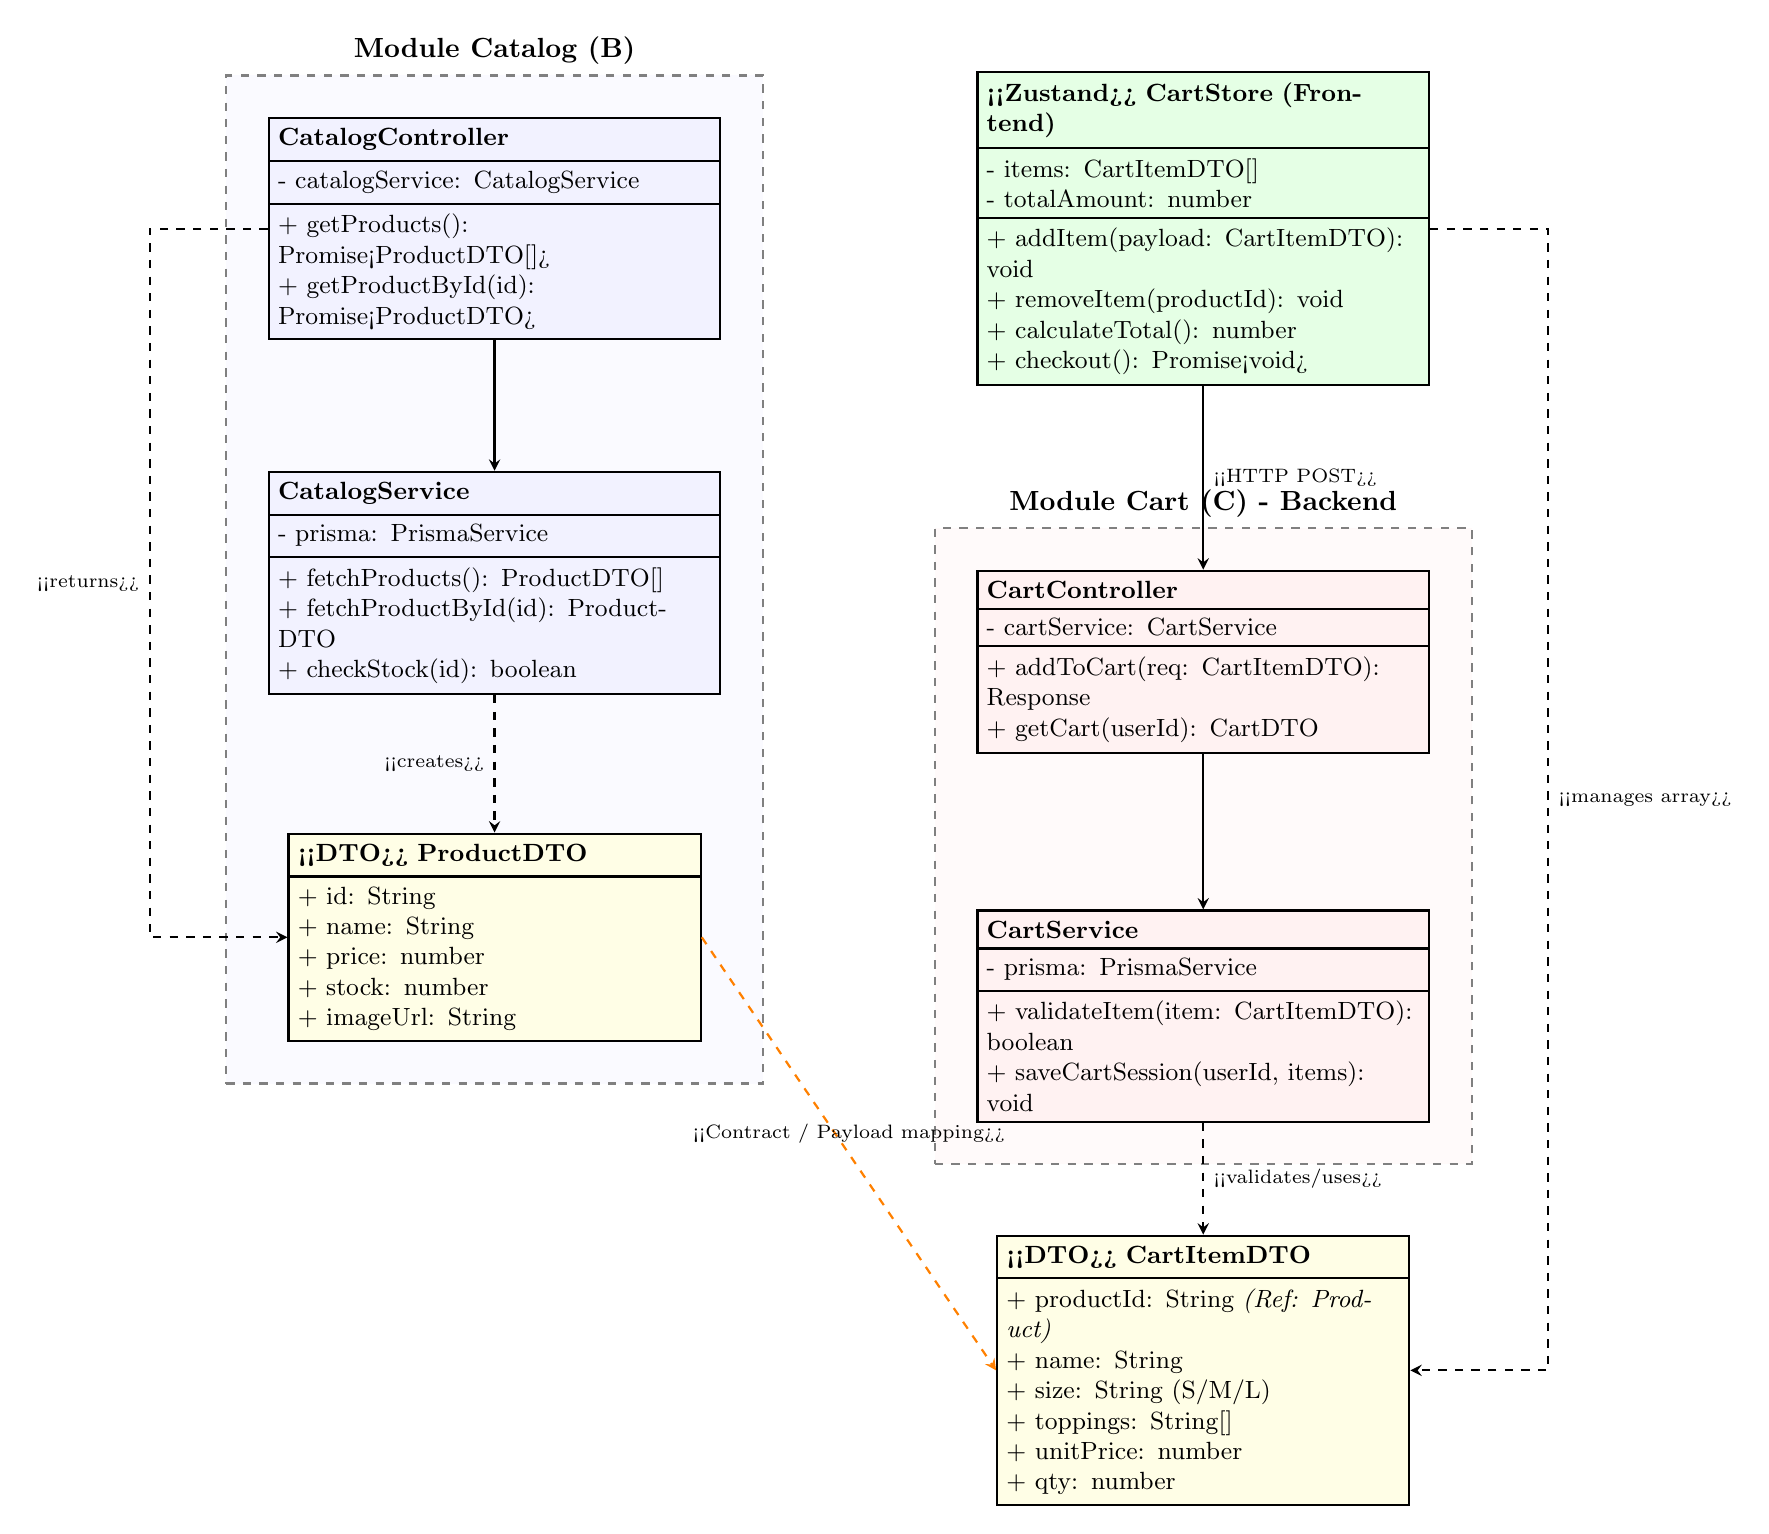
\begin{tikzpicture}[
    >=stealth, thick,
    class/.style={
        rectangle split, rectangle split parts=3,
        draw=black, fill=white, thick,
        text width=5.5cm, align=left,
        font=\small
    },
    dto/.style={
        rectangle split, rectangle split parts=2,
        draw=black, fill=yellow!10, thick,
        text width=5cm, align=left,
        font=\small
    },
    frontend/.style={
        rectangle split, rectangle split parts=3,
        draw=black, fill=green!10, thick,
        text width=5.5cm, align=left,
        font=\small
    },
    relation/.style={->, dashed, thick},
    dependency/.style={->, thick},
    module_box/.style={draw=gray, dashed, thick, inner sep=15pt}
]

% --- MODULE CATALOG (B) ---
\node[class, fill=blue!5] (CatalogController) at (-4, 0) {
    \textbf{CatalogController}
    \nodepart{second}
    - catalogService: CatalogService
    \nodepart{third}
    + getProducts(): Promise<ProductDTO[]>\\
    + getProductById(id): Promise<ProductDTO>
};

\node[class, fill=blue!5] (CatalogService) at (-4, -4.5) {
    \textbf{CatalogService}
    \nodepart{second}
    - prisma: PrismaService
    \nodepart{third}
    + fetchProducts(): ProductDTO[]\\
    + fetchProductById(id): ProductDTO\\
    + checkStock(id): boolean
};

\node[dto] (ProductDTO) at (-4, -9) {
    \textbf{<<DTO>> ProductDTO}
    \nodepart{second}
    + id: String\\
    + name: String\\
    + price: number\\
    + stock: number\\
    + imageUrl: String
};

% --- MODULE CART (C) ---
\node[frontend] (CartStore) at (5, 0) {
    \textbf{<<Zustand>> CartStore (Frontend)}
    \nodepart{second}
    - items: CartItemDTO[]\\
    - totalAmount: number
    \nodepart{third}
    + addItem(payload: CartItemDTO): void\\
    + removeItem(productId): void\\
    + calculateTotal(): number\\
    + checkout(): Promise<void>
};

% FIX LỖI ĐÈ CHỮ: Đẩy các khối dưới thấp xuống 1 bậc
\node[class, fill=red!5] (CartController) at (5, -5.5) {
    \textbf{CartController}
    \nodepart{second}
    - cartService: CartService
    \nodepart{third}
    + addToCart(req: CartItemDTO): Response\\
    + getCart(userId): CartDTO
};

\node[class, fill=red!5] (CartService) at (5, -10) {
    \textbf{CartService}
    \nodepart{second}
    - prisma: PrismaService
    \nodepart{third}
    + validateItem(item: CartItemDTO): boolean\\
    + saveCartSession(userId, items): void
};

\node[dto] (CartItemDTO) at (5, -14.5) {
    \textbf{<<DTO>> CartItemDTO}
    \nodepart{second}
    + productId: String \textit{(Ref: Product)}\\
    + name: String\\
    + size: String (S/M/L)\\
    + toppings: String[]\\
    + unitPrice: number\\
    + qty: number
};

% --- MỐI QUAN HỆ (ARROWS) ---
% Catalog flow
\draw[dependency] (CatalogController) -- (CatalogService);
\draw[relation] (CatalogService) -- node[left, font=\scriptsize] {<<creates>>} (ProductDTO);
\draw[relation] (CatalogController.west) -- ++(-1.5,0) |- node[near start, left, font=\scriptsize] {<<returns>>} (ProductDTO.west);

% Cart flow
\draw[dependency] (CartStore) -- node[right, font=\scriptsize] {<<HTTP POST>>} (CartController);
\draw[dependency] (CartController) -- (CartService);
\draw[relation] (CartService) -- node[right, font=\scriptsize] {<<validates/uses>>} (CartItemDTO);
\draw[relation] (CartStore.east) -- ++(1.5,0) |- node[near start, right, font=\scriptsize] {<<manages array>>} (CartItemDTO.east);

% Cross Module Relationship (Contract)
\draw[relation, draw=orange, thick] (ProductDTO.east) -- node[above, font=\scriptsize, text=black] {<<Contract / Payload mapping>>} (CartItemDTO.west);

% --- BACKGROUND BOUNDARIES ---
\begin{scope}[on background layer]
    \node[module_box, fill=blue!2, fit=(CatalogController) (CatalogService) (ProductDTO)] (catalog_box) {};
    \node[above=0pt of catalog_box, font=\bfseries] {Module Catalog (B)};

    \node[module_box, fill=red!2, fit=(CartController) (CartService)] (cart_box) {};
    \node[above=0pt of cart_box, font=\bfseries] {Module Cart (C) - Backend};
\end{scope}

\end{tikzpicture}
\end{document}